\chapter{Mixture Models}
The real world often generates observable data that falls into a combination of unseen categories. For example, I could record sound waves on a busy street that come from a combination of cars, pedestrians, and animals. If I were to try to model my data points, it would be helpful if I could group them by source, even though I didn't observe where each sound wave came from individually.

In this chapter we explore what are known as mixture models. Their purpose is to handle data generated by a combination of unobserved categories. We would like to discover the properties of these individual categories and determine how they mix together to produce the data we observe. We consider the statistical ideas underpinning mixture models, as well as how they can be used in practice.

\section{Motivation}
Mixture models are used to model data involving \textit{latent variables}.

\begin{definition}{Latent Variable}{latent-variable}
    A latent variable is a piece of data that is not observed, but that influences the observed data. We often wish to create models that capture the behavior of our latent variables.
\end{definition}

We are sometimes unable to observe all the data present in a given system. For example, if we measure the snout length of different animals but only get to see the snout measurements themselves, the latent variable would be the type of animal we are measuring for each data point. For most data generating processes, we will only have access to a portion of the data and the rest will be hidden from us. However, if we can find some way to also model the latent variables, our model will potentially be much richer, and we will also be able to probe it with more interesting questions. To build some intuition about latent variable models, we present a simple directed graphical model with a latent variable $\textbf{z}_n$ in Figure \ref{fig:lvm-dgm}.

\begin{figure}
    \centering
    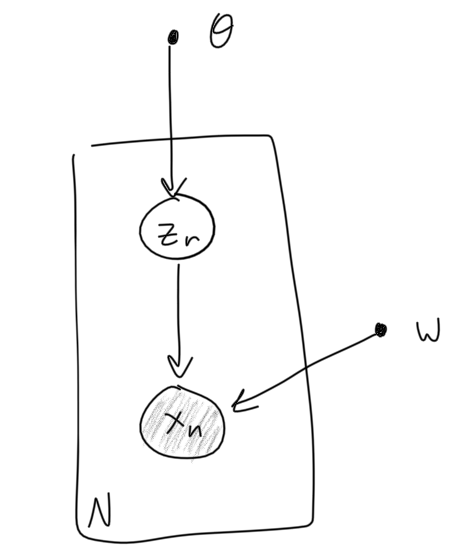
\includegraphics[width=0.3\paperwidth]{../MixtureModels/fig/latent-variable-dgm.png}
    \caption{Directed graphical model with a latent variable $\textbf{z}$.}
    \label{fig:lvm-dgm}
\end{figure}

One common means of modeling data involving latent variables, and the topic of this chapter, is known as a \textit{mixture model}.

\begin{definition}{Mixture Model}{mixture-model}
    A mixture model captures the behavior of data coming from a combination of different distributions.
\end{definition}

At a high level, a mixture model operates under the assumption that our data is generated by first sampling a discrete class, and then sampling a data point from within that category according to the distribution for that category. For the example of animal snouts, we would first sample a species of animal, and then based on the distribution of snout lengths in that species, we would sample an observation to get a complete data point.

Probabilistically, sampling a class (which is our latent variable, since we don't actually observe it) happens according to a Categorical distribution, and we typically refer to the latent variable as $\textbf{z}$. Thus:
\begin{align*}
    p(\textbf{z} = C_{k} ; \boldsymbol{\theta}) = \theta_{k}
\end{align*}
where $C_{k}$ is class $k$, and $\boldsymbol{\theta}$ is the parameter to the Categorical distribution that specifies the probability of drawing each class. Then, once we have a class, we have a distribution for the observed data point coming from that class:
\begin{align*}
    p(\textbf{x} | \textbf{z} = C_{k}; \textbf{w})
\end{align*}
\readernote{The distribution given by $p(\textbf{x} | \textbf{z} = C_{k}; \textbf{w})$ is known as the \textit{class-conditional distribution}.}
This distribution depends on the type of data we are observing, and is parameterized by an arbitrary parameter $\textbf{w}$ whose form depends on what is chosen as the class-conditional distribution. For the case of snout lengths, and many other examples, this conditional distribution will often be Gaussian, in which case our model is known as a \textbf{Gaussian Mixture Model}. We will discuss Gaussian Mixture Models in more detail later in the chapter.

If we can effectively model the distribution of our observed data points and the latent variables responsible for producing the data, we will be able to ask interesting questions of our model. For example, upon observing a new data point $\textbf{x}'$ we will be able to produce a probability that it came from a specific class $\textbf{z}' = C_k$ using Bayes' rule and our model parameters:
\begin{align*}
    p(\textbf{z}' = C_k | \textbf{x}') = \frac{p(\textbf{x}' | \textbf{z}' = C_{k}; \textbf{w})p(\textbf{z}' = C_{k} ; \boldsymbol{\theta})}{\sum_{k'} p(\textbf{x}' | \textbf{z}' = C_{k'}; \textbf{w})p(\textbf{z}' = C_{k'} ; \boldsymbol{\theta})}
\end{align*}
Furthermore, after modeling the generative process, we will be able to generate new data points by sampling from our categorical class distribution, and then from the class-conditional distribution for that category:
\begin{align*}
    \textbf{z} \sim Cat(\boldsymbol{\theta}) \\
    \textbf{x} \sim p(\textbf{x} | \textbf{z} = C_{k}; \textbf{w})
\end{align*}
Finally, it will also be possible for us to get a sense of how many classes our data falls into, if that was not something we were aware of a priori.

\begin{mlcube}{Mixture Models}
While the classes of data in a mixture model will typically be discrete, the class-conditional distribution $p(\textbf{x} | \textbf{z} = C_k)$ can be either discrete or continuous, depending on the form of the data that we observe. Notice also that this is an unsupervised technique: while we have a data set $\textbf{X}$ of observations, our goal is not to make predictions. Rather, we are trying to model the generative process of this data by accounting for the latent variables that generated the data points. Finally, this is a probabilistic model both for the latent variables and for our observed data.
\begin{center}
    \begin{tabular}{c|c|c}
    \textit{\textbf{Domain}} & \textit{\textbf{Training}} & \textit{\textbf{Probabilistic}} \\
    \hline
    Continuous/Discrete & Unsupervised & Yes \\
    \end{tabular}
\end{center}
\end{mlcube}

\section{Applications}
Since most of the data we observe in our world has some sort of unobserved category associated with it, there are a wide variety of applications for mixture models. Here are just a few:
\begin{enumerate}
    \item Handwriting image recognition. The categories are given by the characters (letters, numbers, etc.) and the class-conditional is a distribution over what each of those characters might look like.
    \item Modeling the topics in a document. Words or sentences in a document can be thought of as corresponding to specific topics and the class-condition for a specific topic determines a distribution over the words you might observe for that topic. More on this in the section on LDA at the end of the chapter.
    \item Vehicle prices. Vehicle can be categorized a number of different ways (gas mileage, size, safety, etc.). The class-conditional for a given category determines the distribution over the price of that vehicle.
\end{enumerate}

\section{Fitting a Model}
We've defined the general form of a mixture model: we have a distribution $p(\textbf{z}; \boldsymbol{\theta})$ over our classes and a distribution $p(\textbf{x}|\textbf{z} = C_k; \textbf{w})$ over our class-conditional distribution. A natural approach would be to compute the maximum likelihood values for our parameters $\boldsymbol{\theta}$ and $\textbf{w}$. Let's consider how me might go about this for a mixture model.

\subsection{Maximum Likelihood for Mixture Models}
Our goal is to maximize the likelihood of our observed data. Because we don't actually observe the latent variables $\textbf{z}_n$ which determine the class of each observed data point $\textbf{x}_n$, we can simply sum over the possible classes for each of our $N$ data points as follows:
\begin{align*}
    p(\textbf{X}; \boldsymbol{\theta}, \textbf{w}) = \prod_{n=1}^{N} \sum_{k=1}^{K} p(\textbf{x}_{n}, z_{n, k}; \boldsymbol{\theta}, \textbf{w})
\end{align*}
Taking the logarithm to get our log-likelihood as usual:
\begin{align} \label{intractable-log-likelihood}
    \log p(\textbf{X}; \boldsymbol{\theta}, \textbf{w}) = \sum_{n=1}^{N} \log \bigg[ \sum_{k=1}^{K} p(\textbf{x}_{n}, z_{n, k}; \boldsymbol{\theta}, \textbf{w}) \bigg]
\end{align}
It may not be immediately obvious, but under this setup, the maximum likelihood calculation for our parameters $\boldsymbol{\theta}, \textbf{w}$ is now intractable. The summation over the $K$ classes of our latent variable $\textbf{z}_{n}$, which is required because we don't actually observe those classes, is inside of the logarithm, which prevents us from arriving at a closed form solution (it may be helpful to try to solve this yourself, you'll realize that consolidating a summation inside of a logarithm is not possible). The rest of this chapter will deal with how we can optimize our mixture model in the face of this challenge.

\subsection{Complete-Data Log Likelihood}
We have a problem with computing the MLE for our model parameters. If we only knew which classes our data points came from, we would be able to calculate $\log p(\textbf{x}, \textbf{z})$ with relative ease because we would no longer require a summation inside the logarithm:
\begin{align} \label{complete-data-log-likelihood}
    \log p(\textbf{X}, \textbf{Z}) &= \sum_{n=1}^{N} \log p(\textbf{x}_n, \textbf{z}_n; \boldsymbol{\theta}, \textbf{w}) \\
    &= \sum_{n=1}^{N} \log[p(\textbf{x}_n | \textbf{z}_n = C_k; \textbf{w}) p(\textbf{z}_n = C_k; \boldsymbol{\theta})] \\
    &= \sum_{n=1}^{N} \log p(\textbf{x}_n | \textbf{z}_n = C_k; \textbf{w}) + \log p(\textbf{z}_n = C_k; \boldsymbol{\theta}) \\
\end{align}
Notice that because we've now observed $\textbf{z}_{n}$, we don't have to marginalize over its possible values. This motivates an interesting approach that takes advantage of our ability to work with $p(\textbf{x}, \textbf{z})$ if we only knew $\textbf{z}$.

The expression p(\textbf{x}, \textbf{z}) is known as the \textit{complete-data} because it assumes that we have both our observation $\textbf{x}$ and the classs $\textbf{z}$ that $\textbf{x}$ came from. Our ability to efficiently calculate the complete-data log likelihood $\log p(\textbf{x}, \textbf{z})$ is the crucial piece of the algorithm we will present to optimize our mixture model parameters. This algorithm is known as \textbf{Expectation-Maximization}, or \textbf{EM} for short.

\section{Expectation-Maximization (EM)}
The motivation for the EM algorithm, as presented in the previous section, is that we do not have a closed form optimization for our mixture model parameters due to the summation inside of the logarithm. This summation was required because we didn't observe a crucial piece of data, the class $\textbf{z}$, and therefore we had to sum over its values.

EM uses an iterative approach to optimize our model parameters. It proposes a value for $\textbf{z}$ using an expectation calculation, and then based on that proposed value, it maximizes our complete-data log likelihood with respect to the model parameters $\boldsymbol{\theta}$ and $\textbf{w}$ via a standard MLE procedure.

Notice that EM is composed of two distinct steps: taking an expectation over our latent class variables and performing a maximization over our model parameters. These two steps (expectation and maximization) obviously give the algorithm its name, but more generally, this type of approach is also referred to as \textbf{coordinate ascent}. The idea behind coordinate ascent is that we can replace a hard problem (maximizing the log likelihood for our mixture model directly) with two easier problems (taking an expectation over our latent variables and maximizing our model parameters based on the complete-data, which relies on the current setting of our latent variables). We alternate between the two easier problems, executing each of them until we reach a point of convergence or decide that we've done enough.

We'll walk through the details of each of these two steps and then tie them together with the complete algorithm.

\subsection{Expectation Step}
The purpose of the expectation step (sometimes just referred to as the `E-step') in the EM algorithm is to set the most likely values for our latent variables $\textbf{z}_n$. In an ideal world, we would know what these classes are, and if we did, we could simply optimize our complete-data log likelihood directly as we've seen above. However, since we don't get to observe these values, one way we can get around this is just to compute the expectation of the latent variables. Let's consider what this looks like with a concrete example.

Let's say our data points $\textbf{x}_n$ can come from one of three classes. Then, we can represent the latent variable $\textbf{z}_n$ associated with each data point using a one-hot encoded vector. For example, if $\textbf{z}_n$ came from class $C_1$, we would denote this:
\begin{align*}
    \textbf{z}_n = 
        \begin{bmatrix}
            1 \\
            0 \\
            0 \\
        \end{bmatrix}
\end{align*}
As we've already explained, we don't know the true value of this latent variable. Instead, we will compute its conditional expectation based on the current setting of our model parameters and our observed data $\textbf{x}_n$. We denote the expectation of our latent variables as $\textbf{q}_n$, and we calculate them as follows:
\begin{align*}
    \textbf{q}_n = \mathbb{E}[\textbf{z}_n | \textbf{x}_n] &= \begin{bmatrix}
            p(\textbf{z}_n = C_1 | \textbf{x}_n; \boldsymbol{\theta}, \textbf{w}) \\
            p(\textbf{z}_n = C_2 | \textbf{x}_n; \boldsymbol{\theta}, \textbf{w}) \\
            p(\textbf{z}_n = C_3 | \textbf{x}_n; \boldsymbol{\theta}, \textbf{w}) \\
        \end{bmatrix} \\
        &\propto \begin{bmatrix}
            p(\textbf{x}_n | \textbf{z}_n = C_1; \textbf{w})p(\textbf{z}_n = C_1; \boldsymbol{\theta}) \\
            p(\textbf{x}_n | \textbf{z}_n = C_2; \textbf{w})p(\textbf{z}_n = C_2; \boldsymbol{\theta}) \\
            p(\textbf{x}_n | \textbf{z}_n = C_3; \textbf{w})p(\textbf{z}_n = C_3; \boldsymbol{\theta}) \\
        \end{bmatrix} \\
\end{align*}
Notice that we can switch from proportionality in our $\textbf{q}_n$ values to actually probabilities by simply taking a softmax over the unnormalized values. Then, our $\textbf{q}_n$ values will look something like the following, where a larger number indicates a stronger belief that the data point $\textbf{x}_n$ came from that class:
\begin{align*}
    \textbf{q}_n = \begin{bmatrix}
            0.8 \\
            0.1 \\
            0.1 \\
        \end{bmatrix}
\end{align*}
There are two important things to note about the expectation step. First, the model parameters $\boldsymbol{\theta}$ and \textbf{w} are held fixed. We're computing the expectation of our latent variables based on the current setting of those model parameters. Those parameters are randomly initialized if this is our first time running the expectation step.

Second, notice that we have a value of $\textbf{q}_n$ for every data point $\textbf{x}_n$ in our data set. As a result, $\textbf{q}_n$ are sometimes called \textit{local} variables, since there is one assigned to each data point. This is in contrast to our model parameters $\boldsymbol{\theta}$ and \textbf{w}, which are considered \textit{global} parameters. The size of the global model parameters doesn't fluctuate based on the size of our data set.

After performing the E-step, we now have an expectation for our latent variables, given by $\textbf{q}_n$. In the maximization step, which we describe next, we use these $\textbf{q}_n$ values to optimize our model parameters.

\subsection{Maximization Step}
After the expectation step, we have a $\textbf{q}_n \in \mathbb{R}^K$ associated with each data point $\textbf{x}_n$, which describes our belief that the data point came from each class $C_k$. Now that we have these expected `class assignments', it's possible for us to update our model parameters $\boldsymbol{\theta}$ and $\textbf{w}$.

Recall that optimizing our parameters using the complete-data log likelihood is tractable because we avoid summing over the classes inside of the logarithm. Although we do not have the actual complete-data (we don't know the true $\textbf{z}_n$ values), we have an estimation of the complete-data through our $\textbf{q}_n$ values! We use these values of $\textbf{q}_n$ to make the optimization of our model parameters tractable.

Notice that our $\textbf{q}_n$ values are `soft' assignments - meaning that unlike the $\textbf{z}_n$ values, which are one-hot encodings of assignments to a class, the $\textbf{q}_n$ values have a probability that a data point $\textbf{x}_n$ came from each class. Fortunately, this does not affect our maximization, which starts with out complete-data log likelihood:
\begin{align*}
    \log p(\textbf{X}, \textbf{Z}) = \sum_{n=1}^{N} \log p(\textbf{x}_n | \textbf{z}_n = C_k; \textbf{w}) + \log p(\textbf{z}_n = C_k; \boldsymbol{\theta}) \\
\end{align*}
Applying the expectation with respect to $\textbf{z}_n | \textbf{x}_n$, which will require the $\textbf{q}_n$ computed in the expectation step:
\begin{align} \label{tractable-eqn}
    \mathrm{E}_{\textbf{z}_n | \textbf{x}_n} [\log p(\textbf{X}, \textbf{Z})] &= \mathrm{E}_{\textbf{z}_n | \textbf{x}_n} \bigg[ \sum_{n=1}^{N} \log p(\textbf{x}_n | \textbf{z}_n = C_k; \textbf{w}) + \log p(\textbf{z}_n = C_k; \boldsymbol{\theta}) \bigg] \\
    &= \sum_{n=1}^{N} \mathrm{E}_{\textbf{z}_n | \textbf{x}_n} \bigg[ \log p(\textbf{x}_n | \textbf{z}_n = C_k; \textbf{w}) + \log p(\textbf{z}_n = C_k; \boldsymbol{\theta}) \bigg] \\
    &= \sum_{n=1}^{N} \sum_{k=1}^{K} p(\textbf{z}_n = C_k | \textbf{x}_n) \big( \log p(\textbf{x}_n | \textbf{z}_n = C_k; w) + \log p(\textbf{z}_n = C_k; \boldsymbol{\theta}) \big) \\
    &= \sum_{n=1}^{N} \sum_{k=1}^{K} q_{n, k} \big( \log p(\textbf{x}_n | \textbf{z}_n = C_k; \textbf{w}) + \log p(\textbf{z}_n = C_k; \boldsymbol{\theta}) \big) \\
\end{align}
Notice the crucial difference between this summation and that of Equation \ref{intractable-log-likelihood}: the summation over the classes is now outside of the logarithm! Recall that using the log-likelihood directly was intractable precisely because the summation over the classes was inside of the logarithm. This maximization became possible by taking the expectation over our latent variables (using the values we computed in the E-step), which moved the summation over the classes outside of the logarithm.

We can now complete the M-step by maximizing the tractable Equation \ref{tractable-eqn} with respect to our model parameters $\boldsymbol{\theta}$ and $\textbf{w}$. We simply take the derivative with respect to the parameter of interest, set to 0, solve, and update the parameter with the result.

\subsection{Full EM Algorithm}
Now that we have a grasp on the purpose of the EM algorithm, as well as an understanding of the expectation and maximization steps individually, we are ready to put everything together to describe the entire EM algorithm.

\begin{itemize}
    \item[1.] Begin by initializing our model parameters $\textbf{w}$ and $\boldsymbol{\theta}$, which we can do at random. Since the EM algorithm is performed over a number of iterative steps, we will denote these initial parameter values $\textbf{w}^{(0)}$ and $\boldsymbol{\theta}^{(0)}$. We will increment those values as the algorithm proceeds.
    \item[2.] E-step: compute the values of $\textbf{q}_n$ based on the current setting of our model parameters.
    \begin{align*}
        \textbf{q}_n = \mathbb{E}[\textbf{z}_n | \textbf{x}_n] = \begin{bmatrix}
                p(\textbf{z}_n = C_1 | \textbf{x}_n; \boldsymbol{\theta}^{(i)}, \textbf{w}^{(i)}) \\
                \vdots \\
                p(\textbf{z}_n = C_K | \textbf{x}_n; \boldsymbol{\theta}^{(i)}, \textbf{w}^{(i)}) \\
            \end{bmatrix} 
            \propto \begin{bmatrix}
            p(\textbf{x}_n | \textbf{z}_n = C_1; \textbf{w}^{(i)})p(\textbf{z}_n = C_1; \boldsymbol{\theta}^{(i)}) \\
            \vdots \\
            p(\textbf{x}_n | \textbf{z}_n = C_K; \textbf{w}^{(i)})p(\textbf{z}_n = C_K; \boldsymbol{\theta}^{(i)}) \\
        \end{bmatrix} \\
    \end{align*}
    \item[3.] M-step: compute the values of $\textbf{w}$ and $\boldsymbol{\theta}$ that maximize our expected complete-data log likelihood for the current setting of the values of $\textbf{q}_n$.
    \begin{align*}
        \textbf{w}^{(i + 1)} = \underset{\textbf{w}}{\arg\max} \; \mathbb{E}_{\textbf{q}_n}[\log p(\textbf{X}, \textbf{Z})]
    \end{align*}
    \item[4.] Return to step 2, repeating this cycle until our likelihood converges.
\end{itemize}

\subsection{Connection to K-Means Clustering}
At this point, it's worth considering the similarity between the EM algorithm and another coordinate ascent algorithm that we considered in the context of clustering: K-Means.

Recall that K-Means proceeds according to a similar iterative algorithm: we first make hard assignments of data points to existing cluster centers, and then we update the cluster centers based on the most recent data point assignments.

In fact, the main differences between K-Means clustering and the EM algorithm are that:
\begin{itemize}
    \item[1.] In the EM setting, we make soft cluster assignments through our $\textbf{q}_n$ values, rather than definitively assigning each data point to only one cluster.
    \item[2.] The EM algorithm is able to take advantage of arbitrary probability distributions to capture the behavior of the observed data, whereas K-Means clustering relies only on distance measurements to make assignments and update cluster centers.
\end{itemize}
In summary, K-Means is simply a restricted form of the EM algorithm.

\subsection{Dice Example: Mixture of Multinomials}
Consider the following example scenario: we have two biased dice (with 6 faces) and one biased coin (with 2 sides). Data is generated as follows: first, the biased coin is flipped. If it lands heads, Dice 1 is rolled. If it lands tails, Dice 2 is rolled. We record the result of the dice roll, but that is our only observation. For example, our observations may look like:
\begin{align*}
    1, 5, 3, 4, 2, 2, 3, 1, 6
\end{align*}
We're going to try to infer the parameters of each of the dice based on these observation.

Let's consider how this scenario fits into our idea of a mixture model. First, the latent variable $\textbf{z}_n$ has a natural interpretation as being which dice was rolled for the $n^{th}$ observed data point $\textbf{x}_n$. We can represent $\textbf{z}_n$ using a one-hot vector, so that if the $n^{th}$ data point came from Dice 1, we'd denote that:
\begin{align*}
    \textbf{z}_n =
        \begin{bmatrix}
            1 \\
            0 \\
        \end{bmatrix} \\
\end{align*}
Unsurprisingly, we denote the probability vector associated with the biased coin as $\boldsymbol{\theta} \in \mathbb{R}^{2}$, with $\theta_1$ being the probability of the biased coin landing heads and $\theta_2$ being the probability of the biased coin landing tails.
Furthermore, we need parameters to describe the behavior of our biased dice. We can use $\boldsymbol{\pi_1}, \boldsymbol{\pi}_2 \in \mathbb{R}^{6}$, where each 6-dimensional parameter vector describes the probability that each dice lands on that face. Notice that we now have our model parameters $\textbf{w} = \{\boldsymbol{\theta}, \boldsymbol{\pi}_1, \boldsymbol{\pi}_2 \}$.
Now that we have our model parameters and an understanding of how this problem fits into the mixture model paradigm, we can optimize our model parameters using the EM algorithm.
We start by initializing our parameters $\textbf{w}^{(0)}$.
Next, we need to compute our $\textbf{q}_n$ values (the expectation step). Recall that the formula for this is given by:
\begin{align} \label{E-for-multinomial}
    \textbf{q}_n &= \begin{bmatrix}
                p(\textbf{z}_n = C_1 | \textbf{x}_n; \boldsymbol{\theta}^{(i)}, \textbf{w}^{(i)}) \\
                p(\textbf{z}_n = C_2 | \textbf{x}_n; \boldsymbol{\theta}^{(i)}, \textbf{w}^{(i)}) \\
            \end{bmatrix} \\
            &\propto \begin{bmatrix}
            p(\textbf{x}_n | \textbf{z}_n = C_1; \textbf{w}^{(i)})p(\textbf{z}_n = C_1; \boldsymbol{\theta}^{(i)}) \\
            p(\textbf{x}_n | \textbf{z}_n = C_2; \textbf{w}^{(i)})p(\textbf{z}_n = C_2; \boldsymbol{\theta}^{(i)}) \\
        \end{bmatrix} \\
        &\propto \begin{bmatrix}
            (\pi_{11})^{x_{n,1}}(\pi_{12})^{x_{n,2}}(\pi_{13})^{x_{n,3}}(\pi_{14})^{x_{n,4}}(\pi_{15})^{x_{n,5}}(\pi_{16})^{x_{n,6}}\theta_1 \\
            (\pi_{21})^{x_{n,1}}(\pi_{22})^{x_{n,2}}(\pi_{23})^{x_{n,3}}(\pi_{24})^{x_{n,4}}(\pi_{25})^{x_{n,5}}(\pi_{26})^{x_{n,6}}\theta_2 \\
        \end{bmatrix} \\
\end{align}
where $x_{n,1}, ..., x_{n,6}$ denotes what was rolled for the data point $\textbf{x}_n$.
After computing the values of $\textbf{q}_n$, we are ready to perform the maximization step for our model parameters. Recall that we are maximizing the expected complete-data log likelihood, which takes the form:
\begin{align} \label{M-for-multinomial}
    \mathbb{E}_{\textbf{q}_n}[\log p(\textbf{X}, \textbf{Z})] &= \mathbb{E}_{\textbf{q}_n} \bigg[\sum_{n=1}^{N} \log p(\textbf{z}_n) + \log p(\textbf{x}_n | \textbf{z}_n)\bigg] \\ 
    &= \sum_{n=1}^{N} \mathbb{E}_{\textbf{q}_n} \bigg[ \log p(\textbf{z}_n) + \log p(\textbf{x}_n | \textbf{z}_n)\bigg] \\ 
    &= \sum_{n=1}^{N} \sum_{k=1}^{2} q_{n, k} \bigg( \log \theta_k + \sum_{j=1}^{6} x_{n, j} \log \pi_{k, j} \bigg) \\ 
\end{align}
Note that to maximize the expected complete-data log likelihood, it's necessary to introduce Lagrange multipliers to enforce the constraints $\sum_{k} \theta_k = 1$ and $\sum_{j} \pi_{k, j} = 1$. After doing this, we recover the following update equations for our model parameters:
\begin{align*}
    \theta_{k}^{(i)} \leftarrow \frac{\sum_{n=1}^{N} q_{n, k}}{N}
\end{align*}
\begin{align*}
    \pi_{k}^{(i)} \leftarrow \frac{\sum_{n=1}^{N} q_{n, k} \textbf{x}_{n}}{\sum_{n=1}^{N} \sum_{j=1}^{6} q_{n, k} x_{n, j}}
\end{align*}

We now have everything we need to perform EM for this setup. After initializing our parameters $\textbf{w}^{(0)}$, we perform the E-step by evaluating \ref{E-for-multinomial}. After calculating our values of $\textbf{q}_n$ in the E-step, we update our parameters $\textbf{w} = \{\boldsymbol{\theta}, \boldsymbol{\pi}_1, \boldsymbol{\pi}_2 \}$ in the M-step by maximizing \ref{M-for-multinomial} with respect to $\boldsymbol{\theta}, \boldsymbol{\pi}_1, \boldsymbol{\pi}_2$. We perform these two steps iteratively, until convergence of our parameters.

\section{Gaussian Mixture Models (GMM)}
Our previous example was a simple but somewhat restricted application of the EM algorithm to solving a latent variable problem. We now turn to a more practical example, used widely in different contexts, called a Gaussian Mixture Model (GMM). As you might expect, a GMM consists of a combination of multiple Gaussian distributions. Among other things, it is useful for modeling scenarios where the observed data is continuous.

Let's go over a more rigorous formulation of the GMM setup. First, we have observed continous data $\textbf{x}_n \in \mathbb{R}^{m}$ and latent variables $\textbf{z}_n$ which indicate which Gaussian `cluster' our observed data point was drawn from. In other words:
\begin{align*}
    p(\textbf{x}_n | \textbf{z}_n = C_k) = \mathcal{N}(\textbf{x}_n; \boldsymbol{\mu}_k, \boldsymbol{\Sigma}_k)
\end{align*}
where $\boldsymbol{\mu}_k, \boldsymbol{\Sigma}_k$ are the mean and covariance parameters respectively for the $k^{th}$ cluster center.

The data generation process works as follows: we first sample a cluster center from a Categorical distribution parameterized by $\boldsymbol{\theta} \in \mathrm{R}^{K}$. Then, based on the sampled cluster center, we sample a data point $\textbf{x}_n \in \mathrm{R}^{m}$, which is the only piece of data that we actually observe. As usual for a mixture model, it is our goal to use the observed data to determine the cluster means and covariances, as well as the parameters of the Categorical distribution that selects the cluster centers.

Fortunately, this problem setup is perfectly suited for EM. We can apply the same machinery we've discussed throughout the chapter and used in the previous example.
\begin{itemize}
    \item[1.] First, we randomly initialize our parameters $\boldsymbol{\theta}, \{ \boldsymbol{\mu}_k, \boldsymbol{\Sigma}_k \}_{k=1}^{K}$.
    \item[2.] [E-Step] Calculate the posterior distribution over $\textbf{z}_n$ given by $\textbf{q}_n$:
        \begin{align*}
            \textbf{q}_n = \mathrm{E}[\textbf{z}_n | \textbf{x}_n] &= \begin{bmatrix}
                p(\textbf{z}_n = C_1 | \textbf{x}_n; \theta_1, \boldsymbol{\mu}_1, \boldsymbol{\Sigma}_1) \\
                \vdots \\
                p(\textbf{z}_n = C_K | \textbf{x}_n; \theta_K, \boldsymbol{\mu}_K, \boldsymbol{\Sigma}_K) \\
            \end{bmatrix} \\
            &\propto \begin{bmatrix}
                \theta_1 \mathcal{N}(\textbf{x}_n; \boldsymbol{\mu}_1, \boldsymbol{\Sigma}_1) \\
                \vdots \\
                \theta_K \mathcal{N}(\textbf{x}_n; \boldsymbol{\mu}_K, \boldsymbol{\Sigma}_K) \\
            \end{bmatrix} \\
        \end{align*}
        This is the current expectation for our latent variables $\textbf{z}_n$ given our data $\textbf{x}_n$ and the current setting of our model parameters $\boldsymbol{\theta}, \{ \boldsymbol{\mu}_k, \boldsymbol{\Sigma}_k \}_{k=1}^{K}$.
    \item[3.] [M-Step] Using our values of $\textbf{q}_n$, calculate the expected complete-data log likelihood, and then use that term to optimize our model parameters:
        \begin{align*}
            \mathbb{E}_{\textbf{q}_n}[\log p(\textbf{X}, \textbf{Z})] &= \mathbb{E}_{\textbf{q}_n} \bigg[ \sum_{n=1}^{N} \ln(p(\textbf{x}_n, \textbf{z}_n; \boldsymbol{\theta}, \{ \boldsymbol{\mu}_k, \boldsymbol{\Sigma}_k \}_{k=1}^{K})) \bigg] \\
            &= \sum_{n=1}^{N} \sum_{k=1}^{K} q_{n, k} \ln \theta_k + q_{n, k} \ln \mathcal{N}(\textbf{x}_n; \boldsymbol{\mu}_k, \boldsymbol{\Sigma}_k) \\
        \end{align*}
        We can then use this expected complete-data log likelihood to optimize our model parameters $\boldsymbol{\theta}, \{ \boldsymbol{\mu}_k, \boldsymbol{\Sigma}_k \}_{k=1}^{K}$ by computing the MLE as usual. Using a Lagrange multiplier to enforce $\sum_{k=1}^{K} \theta_k = 1$, we recover the update equations:
        \begin{align*}
            \theta_k^{(i + 1)} &\leftarrow \frac{\sum_{n=1}^{N} q_{n, k}}{N} \\
            \boldsymbol{\mu}_k^{(i + 1)} &\leftarrow \frac{\sum_{n=1}^{N} q_{n, k} \textbf{x}_n}{\sum_{n=1}^{N} q_{n, k}} \\
            \boldsymbol{\Sigma}_k^{(i + 1)} &\leftarrow \frac{\sum_{n=1}^{N} q_{n, k} (\textbf{x}_n - \boldsymbol{\mu}_k^{(i + 1)})(\textbf{x}_n - \boldsymbol{\mu}_k^{(i + 1)})^{T}}{\sum_{n=1}^{N} q_{n, k}} \\
        \end{align*}
    \item[4.] Return to step 2. Repeat until convergence.
\end{itemize}

Finally, it's worth considering the similarity between GMMs and K-Means clustering. First, as discussed previously, GMMs rely on soft assignments rather than hard assignments. Additionally, GMMs define a normal distribution over our clusters, as opposed to a fixed point in K-Means. Intuitively, K-Means is comparable to a GMM where we only allow hard assignments and the distribution over our clusters is infinitely peaked (meaning our clusters have variance that approaches 0). In other words, K-Means is just a special case of GMMs where we've imposed more rigorous constaints than are ordinarily required by a GMM.

\section{Admixture Models: Latent Dirichlet Allocation (LDA)}
With a grasp on mixture models, it is not too difficult to understand admixture models. In a sentence: an admixture model is a mixture of mixture models. Latent Dirichlet Allocation (LDA) is a common form of admixture models, and it is sometimes also referred to as \textit{topic modeling}, for reasons that will become apparent shortly. Describing LDA using an example will hopefully make the idea of an admixture model more concrete.

\subsection{LDA for Topic Modeling}
Consider the following data generating process for a set of text documents. We have a Dirichlet distribution $\boldsymbol{\theta} \sim Dir(\boldsymbol{\alpha})$ over the possible topics a document can take on.

\readernote{If you haven't seen the Dirichlet before, it is a distribution over an $n$-dimensional vector whose components sum to 1. For example, a sample from a dirichlet distribution in 3-dimensions could produce a sample that is the vector $$\begin{bmatrix} 0.2 \\ 0.5 \\ 0.3 \\ \end{bmatrix}$$.}

We sample from that Dirichlet distribution to determine the mixture of topics $\boldsymbol{\theta}_n$ in our document $D_n$:
\begin{align*}
    \boldsymbol{\theta}_n \sim Dir(\boldsymbol{\alpha})
\end{align*}
Then, for each possible topic, we sample from a Dirichlet distribution to determine the mixture of words $\boldsymbol{\phi}_k$ in that topic:
\begin{align*}
    \boldsymbol{\phi}_k \sim Dir(\boldsymbol{\beta})
\end{align*}
Then, for each word $\textbf{w}_{n, j}$ in the document $D_n$, we first sample from a Categorical parameterized by the topic mixture $\boldsymbol{\theta}_n$ to determine which topic that word will come from:
\begin{align*}
    \textbf{z}_{n, j} \sim Cat(\boldsymbol{\theta}_n)
\end{align*}
Then, now that we have a topic given by $\textbf{z}_{n, j}$ for this word $\textbf{w}_{n, j}$, we sample from a Categorical parameterized by that topic's mixture over words given by $\boldsymbol{\phi}_{\textbf{z}_{n, j}}$:
\begin{align*}
    \textbf{w}_{n, j} \sim Cat(\boldsymbol{\phi}_{\textbf{z}_{n, j}})
\end{align*}

Notice the mixture of mixtures at play here: we have a mixture model over the topics to produce each document in our corpus, and then for every word in a given document, we have a mixture over the topics to generate each individual word.

The indexing is particularly confusing because there are several layers of mixtures here, but to clarify: $n \in 1..N$ indexes each document $D_n$ in our corpus, $k \in 1..K$ indexes each possible topic, and $j \in 1..J$ indexes each word $\textbf{w}_{n,j}$ in document $D_n$, and $e \in 1..E$ indexes each word in our dictionary (note that $\textbf{w}_{n,j} \in \mathbb{R}^{E}$).

$\boldsymbol{\theta}_n$ specifies the distribution over topics in document $D_n$, and $\boldsymbol{\alpha}$ is the hyperparameter for the distribution that produces $\boldsymbol{\theta}_n$. Similarly, $\boldsymbol{\phi}_k$ specifies the distribution over words for the $k^{th}$ topic, and $\boldsymbol{\beta}$ is the hyperparameter for the distribution that produces $\boldsymbol{\phi}_k$.

\subsection{Applying EM to LDA}
Now that the problem setup and notation are taken care of, let's consider how we can apply EM to optimize the parameters $\boldsymbol{\theta}_n$ (the mixture over topics in a document) and $\boldsymbol{\phi}_k$ (the mixture over words for a topic). Note that we can simplify the problem slightly by considering $\boldsymbol{\theta}_n$ and $\boldsymbol{\phi}_k$ to be deterministic parameters for optimization (rather than random variables parameterized by $\boldsymbol{\alpha}$ and $\boldsymbol{\beta}$). Then, EM proceeds as follows:

\begin{itemize}
    \item[1.] First, we randomly initialize our parameters \{$\boldsymbol{\theta}_n \}_{n=1}^{N}, \{ \boldsymbol{\phi}_k\}_{k=1}^{K}$.
    \item[2.] [E-Step] Fix the topic distribution of the document given by $\boldsymbol{\theta}_n$ and the word distribution under a topic given by $\boldsymbol{\phi}_k$. Calculate the posterior distribution $\textbf{q}_{n, j} = p(\textbf{z}_{n, j} | \textbf{w}_{n, j})$, and note that this is the distribution over the possible topics of a word:
        \begin{align*}
            \textbf{q}_{n, j} = \mathrm{E}[\textbf{z}_{n, j} | \textbf{w}_{n, j}] &= \begin{bmatrix}
                p(\textbf{z}_{n, j} = C_1 | \textbf{w}_{n, j}; \boldsymbol{\theta}_n, \boldsymbol{\phi}_1) \\
                \vdots \\
                p(\textbf{z}_{n, j} = C_K | \textbf{w}_{n, j}; \boldsymbol{\theta}_n, \boldsymbol{\phi}_K) \\
            \end{bmatrix} \\
            &\propto \begin{bmatrix}
                p(\textbf{w}_{n, j} | \textbf{z}_{n, j} = C_1; \boldsymbol{\phi}_1) p(\textbf{z}_{n, j}  = C_1; \boldsymbol{\theta}_n) \\
                \vdots \\
                p(\textbf{w}_{n, j} | \textbf{z}_{n, j} = C_K; \boldsymbol{\phi}_K) p(\textbf{z}_{n, j}  = C_K; \boldsymbol{\theta}_n) \\
            \end{bmatrix} \\
            &= \begin{bmatrix}
                \phi_{1, \textbf{w}_{n, j}} \cdot \theta_{n, 1} \\
                \vdots \\
                \phi_{K, \textbf{w}_{n, j}} \cdot \theta_{n, K} \\
            \end{bmatrix} \\
        \end{align*}
    \item[3.] [M-Step] Using our values of $\textbf{q}_n$, calculate the expected complete-data log likelihood (which marginalizes over the unknown hidden variables $\textbf{z}_{n, j}$), and then use that expression to optimize our model parameters $\boldsymbol{\theta}_n$ and $\boldsymbol{\phi}_k$:
        \begin{align*}
            \mathbb{E}_{\textbf{q}_n}[\log p(\textbf{W}, \textbf{Z})] &= \mathbb{E}_{\textbf{q}_n} \bigg[ \sum_{n=1}^{N} \sum_{j=1}^{J} \ln(p(\textbf{w}_{n, j}, \textbf{z}_{n, j}; \{\boldsymbol{\theta}_n \}_{n=1}^{N}, \{ \boldsymbol{\phi}_k\}_{k=1}^{K} \bigg] \\
            &= \sum_{n=1}^{N} \sum_{j=1}^{J} \sum_{k=1}^{K} q_{n, j, k} \ln \theta_{n, k} + q_{n, j, k} \ln \phi_{k, \textbf{w}_{n, j}} \\
        \end{align*}
        We can then use this expected complete-data log likelihood to optimize our model parameters $\{\boldsymbol{\theta}_n \}_{n=1}^{N}, \{ \boldsymbol{\phi}_k\}_{k=1}^{K}$ by computing the MLE as usual. Using Lagrange multipliers to enforce $\forall n \sum_{k=1}^{K} \theta_{n, k} = 1$ and $\forall k \sum_{e=1}^{E} \phi_{k, e} = 1$ (where $e$ indexes each word in our dictionary), we recover the update equations:
        \begin{align*}
            \theta_{n, k}^{(i + 1)} &\leftarrow \frac{\sum_{j=1}^{J} q_{n, j, k}}{J} \\
            \phi_{k, d}^{(i + 1)} &\leftarrow \frac{\sum_{n=1}^{N} \sum_{j=1}^{J} q_{n, j, k} w_{n, j, d}}{\sum_{n=1}^{N} \sum_{j=1}^{J} q_{n, j, k}} \\
        \end{align*}
    \item[4.] Return to step 2. Repeat until convergence.
\end{itemize}

The largest headache for applying the EM algorithm to LDA is keeping all of the indices in order, and this is the result of working with a mixture of mixtures. Once the bookkeeping is sorted out, the actual updates are straightforward.

\section{Conclusion}
Mixture models are one common way of handling data that we believe is generated through a combination of unobserved, latent variables. We've seen that training these models directly is intractable (due to the marginalization over the latent variables), and so we turned to a coordinate ascent based algorithm known as Expectation-Maximization to get around this difficulty. We then explored a couple of common mixture models, including a multinomial mixture, Gaussian Mixture Model, and an admixture model known as Latent Dirichlet Allocation. Mixture models are a subset of a broader range of models known as latent variable models, and the examples seen in this chapter are just a taste of the many different mixture models available to us. Furthermore, EM is just a single algorithm for optimizing these models. A good grasp on the fundamentals of mixture models and the EM algorithm will be useful background for expanding to more complicated, expressive latent variable models.
